\subsection*{Teil A: Eigenschaften von Vierecken erkennen (25 Minuten)}

\begin{enumerate}[label=\arabic*.]

    \item \textbf{Ordne die Vierecke ihren Namen zu:}

    \vspace{0.5cm}
    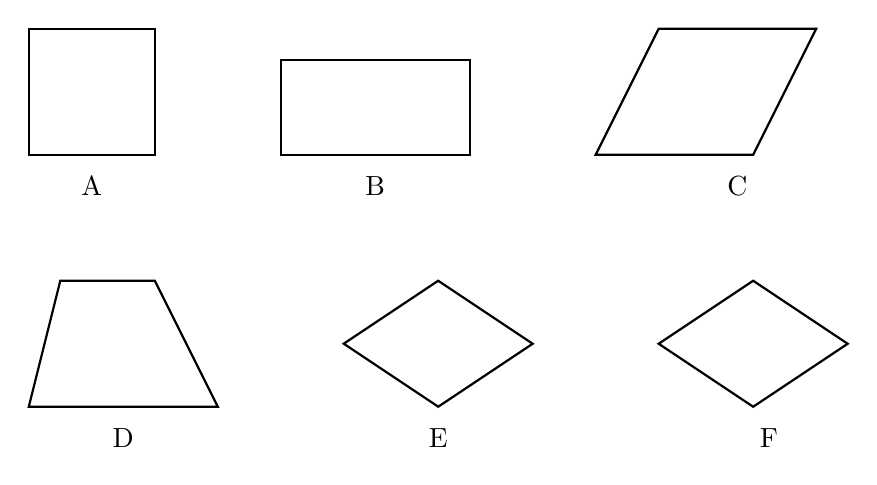
\begin{tikzpicture}[scale=0.8]
        % Quadrat
        \draw[thick] (0,0) rectangle (2,2);
        \node at (1,-0.5) {A};

        % Rechteck
        \draw[thick] (4,0) rectangle (7,1.5);
        \node at (5.5,-0.5) {B};

        % Parallelogramm
        \draw[thick] (9,0) -- (11.5,0) -- (12.5,2) -- (10,2) -- cycle;
        \node at (11.25,-0.5) {C};

        % Trapez
        \draw[thick] (0,-4) -- (3,-4) -- (2,-2) -- (0.5,-2) -- cycle;
        \node at (1.5,-4.5) {D};

        % Raute
        \draw[thick] (5,-3) -- (6.5,-2) -- (8,-3) -- (6.5,-4) -- cycle;
        \node at (6.5,-4.5) {E};

        % Drachenviereck
        \draw[thick] (10,-3) -- (11.5,-2) -- (13,-3) -- (11.5,-4) -- cycle;
        \node at (11.75,-4.5) {F};
    \end{tikzpicture}

    \vspace{0.5cm}
    Verbinde mit Linien:
    \begin{center}
        \begin{tabular}{ll}
            Quadrat & \hspace{3cm} Figur \_\_\_ \\[0.5cm]
            Rechteck & \hspace{3cm} Figur \_\_\_ \\[0.5cm]
            Parallelogramm & \hspace{3cm} Figur \_\_\_ \\[0.5cm]
            Trapez & \hspace{3cm} Figur \_\_\_ \\[0.5cm]
            Raute & \hspace{3cm} Figur \_\_\_ \\[0.5cm]
            Drachenviereck & \hspace{3cm} Figur \_\_\_ \\
        \end{tabular}
    \end{center}

    \vspace{1cm}

    \item \textbf{Eigenschaften markieren:}

    Kreuze bei jedem Viereck die zutreffenden Eigenschaften an:

    \begin{center}
        \begin{tabular}{|p{3cm}|c|c|c|c|c|}
            \hline
            \textbf{Eigenschaft} & \textbf{Quadrat} & \textbf{Rechteck} & \textbf{Raute} & \textbf{Parallelogramm} & \textbf{Trapez} \\
            \hline
            Alle Seiten gleich lang & $\square$ & $\square$ & $\square$ & $\square$ & $\square$ \\
            \hline
            Gegenüberliegende Seiten parallel & $\square$ & $\square$ & $\square$ & $\square$ & $\square$ \\
            \hline
            Alle Winkel 90° & $\square$ & $\square$ & $\square$ & $\square$ & $\square$ \\
            \hline
            Diagonalen gleich lang & $\square$ & $\square$ & $\square$ & $\square$ & $\square$ \\
            \hline
            Diagonalen halbieren sich & $\square$ & $\square$ & $\square$ & $\square$ & $\square$ \\
            \hline
        \end{tabular}
    \end{center}

\end{enumerate}